\documentclass[12pt]{article}
\usepackage[utf8]{inputenc}
\usepackage{chemfig}
\usepackage[version=4]{mhchem}
\usepackage{amsfonts}
\usepackage{amsmath}
\usepackage{amssymb}
\usepackage{geometry}
\usepackage{mathabx}
\usepackage{relsize}
\usepackage{graphics}
\usepackage{outlines}
\usepackage[colorlinks = true,
            linkcolor = blue,
            urlcolor  = blue,
            citecolor = blue,
            anchorcolor = blue]{hyperref}
%\usepackage{indentfirst}
\usepackage{tikz}
\usepackage{listings}
\usepackage{sidecap}
\usepackage{comment}
\geometry{
 a4paper,
 total={6.5in,0in},
 left= 15mm,
 top= 15mm,
 bottom=15mm,
 right = 15mm
 }
\title{Energy Log}
\author{Marcos Perez}
\date{June 2022 - }

\begin{document}

\maketitle

\section{June-ish}
\subsubsection{5/31/22}
Configuring \href{https://docs.github.com/en/repositories/working-with-files/managing-large-files/configuring-git-large-file-storage}{https://docs.github.com/en/repositories/working-with-files/managing-large-files/configuring-git-large-file-storage}\\
Currently pushing some datasets to the Github repository. \\
It worked! :)\\
Note from the future (7/25) I went way past the 5 GB maximum and decided to delete it. Will instead use a Google Drive account to host all the data as a back up.
\subsubsection{6/13/2022}
Downloaded ENDF-Libraries. Extracting all of the files from subfolders automatically using 7-zip :)\\
Added the page where I downloaded everything to list of links. Trying the EMPIRE software for simulations to see if its helpful. I suspect it will be. \\
Ended up deleting it because I don't think it will be useful. \\
Downloaded \href{https://www.nist.gov/pml/atomic-weights-and-isotopic-compositions-relative-atomic-masses}{isotopic abundances} from the National Institute of Standards and Technology. 
\subsection{6/27/2022}
I should do math using Sage Notebooks Using the gruvbox theme in sage :) \\
\subsubsection{6/30/22}
Just had a meeting with Bethany. I could include the shielding in the mass by keeping track of the radiation type and their contribution to the power density. \\
Now that I've been using a variety of tools for data analysis and computational physics, I've decided the following are the advantages of each:
\begin{itemize}
    \item Speed, ease of use - Julia
    \item Package ecosystem, ease of use - Python (pypy can yield some speed improvements but will always lag behind Julia)
    \item Colab - make jupyter notebooks more accessible and easily shared
    \item Git + Github - use it. The desktop version is more user friendly and thorough but less reliable. For more straightforward applications, the command line version is faster and more than worth setting up for long term projects. 
    \item Streamlit - for interactive data visualizations you want to exist in the world, this is much easier to use than Heroku. 
    \item Heroku - longer lived than streamlit, and I suspect will outlive it. 
    \item Dash + Plotly - awesome in Python, needs some work in Julia. 
\end{itemize}

Since I already have the beta decay fraction, maybe I could just filter out the isotopes that can directly emit non-beta radiation? It's so hard to go between all these files. I should write down the whole process as a flow chart and put it into a singular notebook. \\
Did that for decay chains that only decay via beta decay. Have to refine to exclude gammas and unstable daughter products. Need to repeat for all decay types. Shielding!\\
\section{July}
\subsubsection{7/5/2022}
Making a functional backup on colab \href{https://colab.research.google.com/drive/1rXPnMapuznZOmF3p908jdk1eiosalbjV?usp=sharing}{https://colab.research.google.com/drive/1rXPnMapuznZOmF3p908jdk1eiosalbjV?usp=sharing}\\

What is the decay energy I've been using the power densities? It should be the sum of the beta decay and any gamma emissions. Do the project multiple ways until and see how much the results agree.\\
Finally found a way to describe my project: simulating radioisotope production for energy storage. Data driven optimization of nuclear medicine. 
\textbf{Different Analyses and Data Sources}
\begin{enumerate}
    \item \href{https://www-nds.iaea.org/amdc/}{Nubase 2020 + AME 2020} + \href{https://nds.iaea.org/relnsd/vcharthtml/api_v0_guide.html}{Livechart} $\to$ decay chains with any of the following decay modes: \\
    a: alpha decay beta plus decay and electron capture, bm: beta minus decay, g: gamma emission, e: Auger and conversion electron, x: X-ray emission
    \item \href{https://www-nds.iaea.org/amdc/}{Nubase 2020 + AME 2020} + \href{https://www.doseinfo-radar.com/RADARDecay.html}{RADAR} $\to$ decay chains that only include the decay modes $\beta^-$ decay and gamma emission (except for the final daughter nucleus, which can decay by any mode or even be stable).
\end{enumerate}
The only thing standing between seamlessly using the same code on Colab and my laptop is the file system. I need to write a function to handle that. Left off in the livecharts notebook on Github and the laptop and  \href{https://colab.research.google.com/drive/1rXPnMapuznZOmF3p908jdk1eiosalbjV?usp=sharing}{this colab notebook}\\
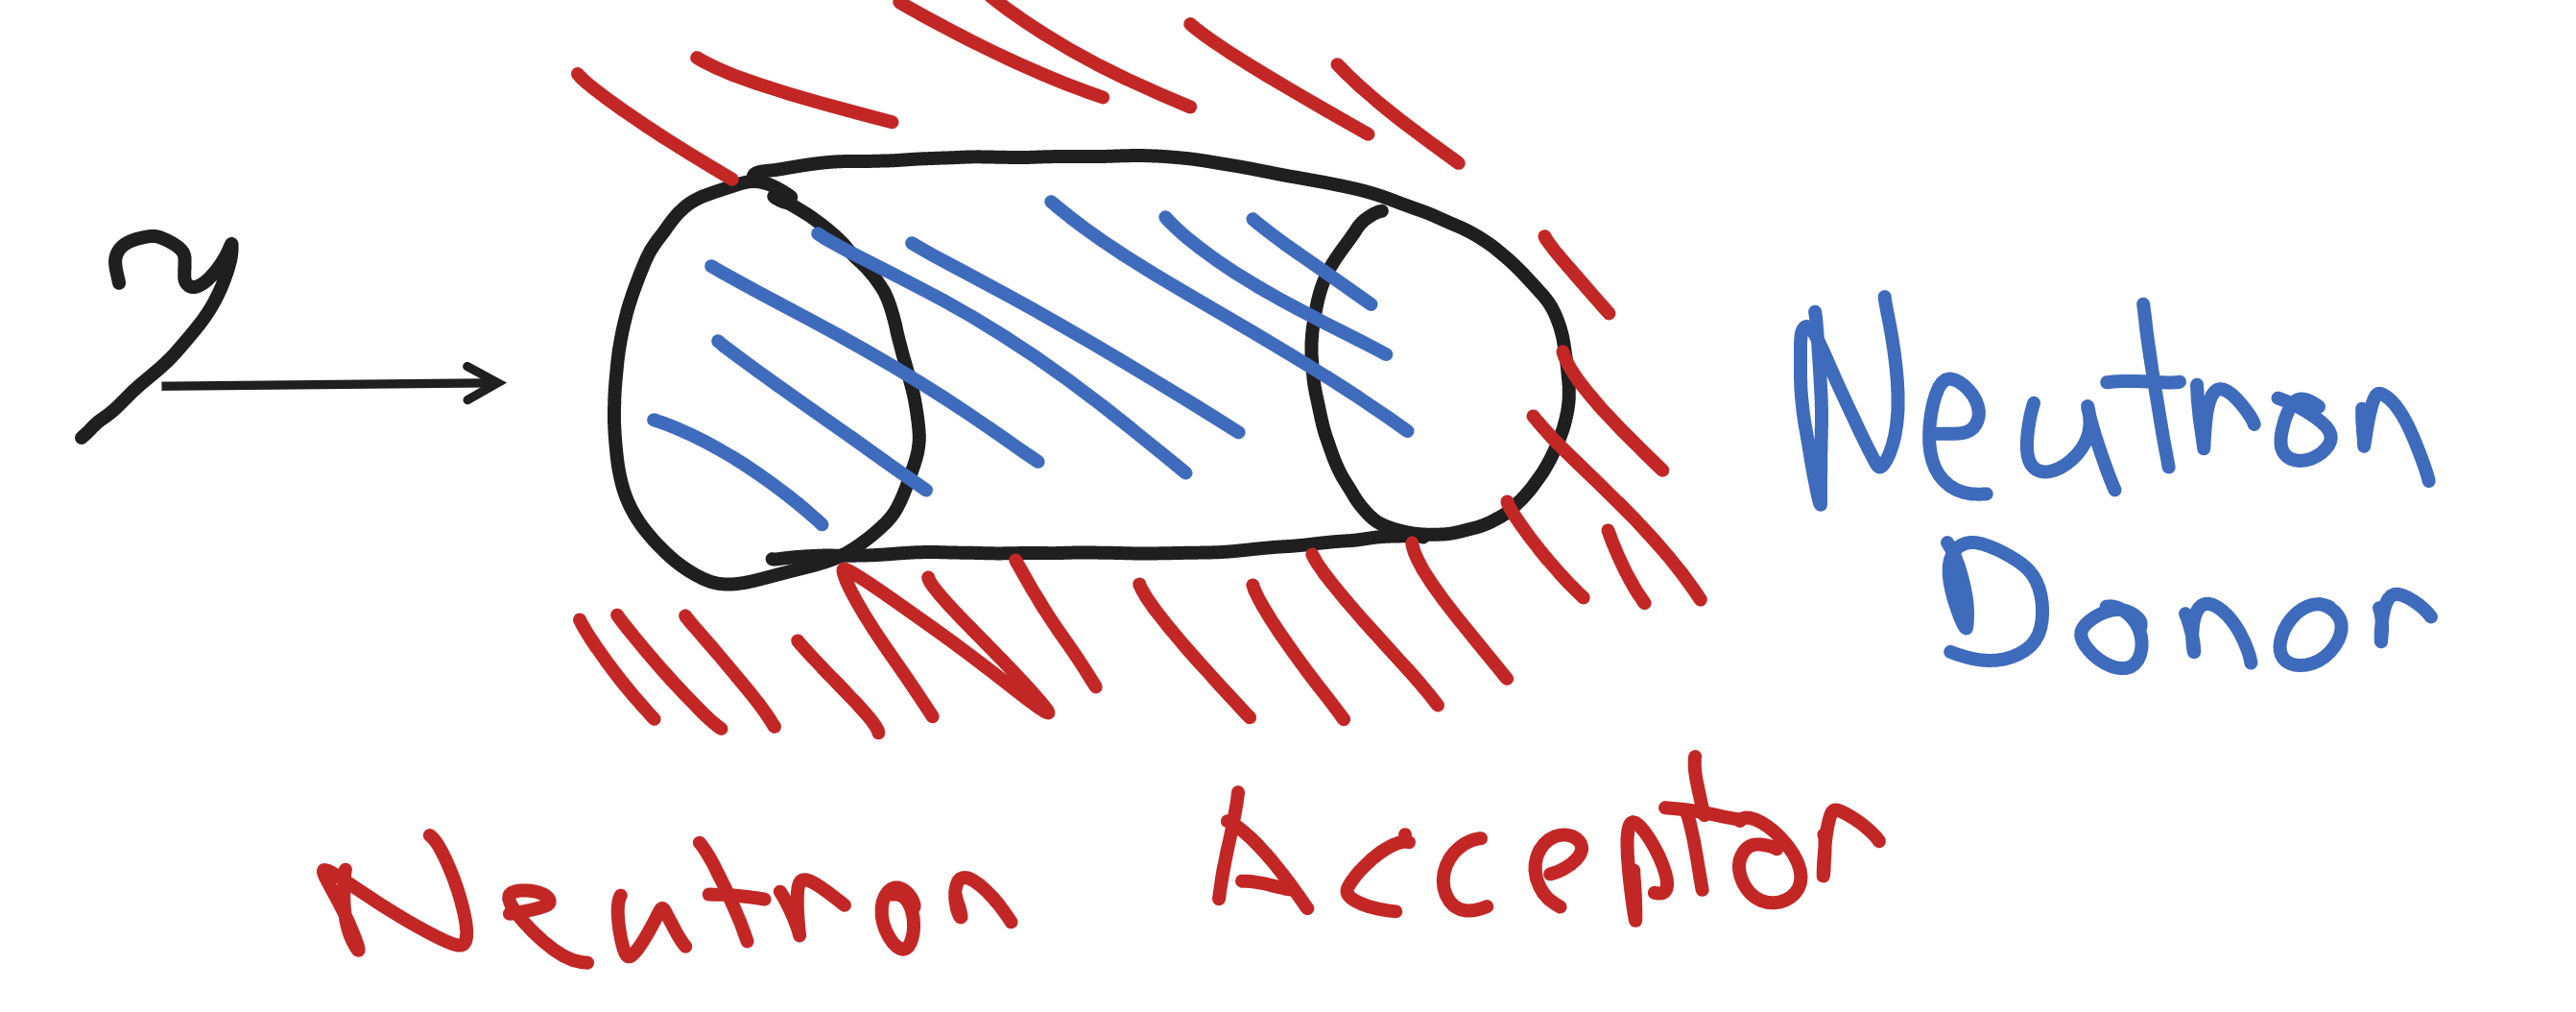
\includegraphics[scale=.4]{Images/concept setup.PNG}\\
In this setup, a gamma ray will be fired at a neutron donor (blue cylinder) which would then be captured by the neutron acceptor (red surroundings). Ideally, the neutron donor would have a very small radius but be a very long cylinder. Assuming every gamma ray produces a neutron which is then capture by the neutron acceptor, it would only cost 1 MeV/neutron with deuterium as a neutron donor (leading an energy storage efficiency of $~\frac{1}{3}$ based on the power density of decay chains work since one traverse along each chain yields $300$ keV). Can it's low cross section and density be overcome with this design? What is the ideal neutron acceptor for each neutron donor? Is this less efficient than firing protons into the neutron acceptor? 
\subsubsection{7/25/2022}
Found the readmes for the complete data libraries and found the most recent libraries \\
\subsubsection{7/26}
Doing more data wrangling using the link with the superset of all the data in the list of links file. Will combine all of the data into a singular directory for each projectile. 
\section{August}
\subsubsection{8/9/2022}
Installed and setup talys in a subdirectory of my downloads folder using WSL. In the process, I downloaded gfortran. Now have a talys executable in the bin directory of WSL. \\
Also automated and the use of the DPASS GUI to retrieve data. Takes $<$ 6 hours to retrieve the entire database. \\

\subsubsection{8/11/2022}
Made a lot more progress on the code. Wondering if radiative capture and neutron absorption are the only two competing reactions? They are certianly a subset of them. (screenshot from endf6 manual) \\
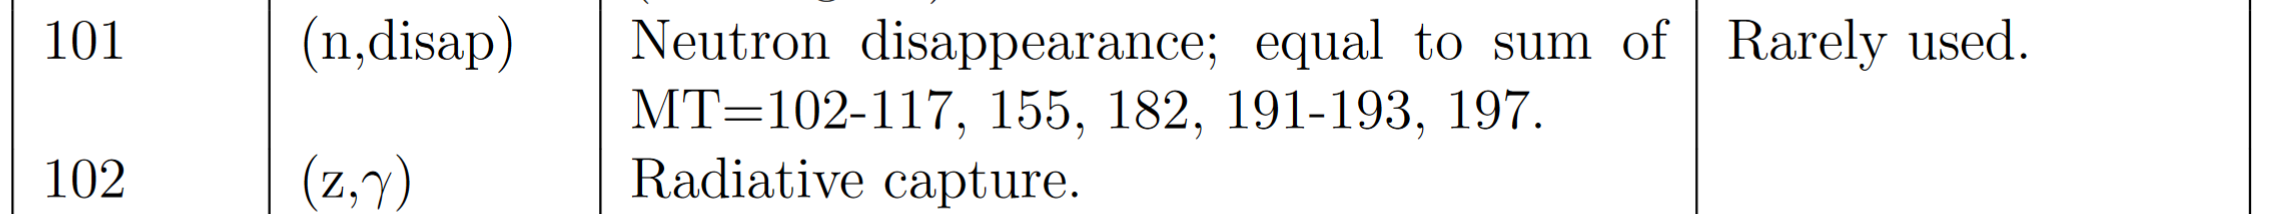
\includegraphics[scale=.4]{Images/are these the only two competing reactions.PNG}\\
I don't care about the specific reaction so much as the residual products including the desired product isotope. 

\subsubsection{8/15/2022}
Been reading \href{https://www-nds.iaea.org/exfor}{exfor} a lot recently. \\
very pleasantly surprised by some of the gamma ray cross sections of Fe-58. On the order of .001 barns at .01 MeV for the emission a neutron. We have 
\begin{equation}
    k = \frac{\rho\sigma N_A}{M}
\end{equation}
where $M$ is the molar mass in kg, $N_A$ is Avogadro's constant, $\sigma$ is the cross section in m$^2$ and $\rho$ is the mass density in kg/m$^3$. Note that for iron, $\rho N_A/M\approx 6\times10^{26}$.
Based on "On the 58Fe($\gamma$,n)57Fe reaction near a threshold" by Kitaev et al, there is a surprisingly low energy peak of 0.038 barns at 0.00597 MeV. 
$k\approx  6\sigma\times10^{26} approx  10^{-3}$. Thus, for a \textbf{thin} target it would take approximately 6 MeV to produce each neutron. Either the data is wrong or I am reading it wrong (maybe it is actually meant to be in GeV??). According to both ENDF and TENDL, it cross sections should peak at .096 barns at 19 MeV, which makes much more since when considering the nuclear binding energy that must be overcome in the $(\gamma,n)$ reaction. 
\subsubsection{August 26th}
After months of consideration I've decided on the following for my workflow: 
\begin{outline}
\1 Repetitive or computationally expensive tasks
    \2 Code these parts using the Julia language rather than Python. While I'm writing it, I can even do so in a Jupyter notebook, I just need to set the kernel to the Julia executable. There is a shortcut to do exactly this in VS code, so it is very convenient to go between kernels. 
    \2 By uploading such a notebook to Google Colab, then downloading it as a .py file, then resaving it as a .jl file, it is very fast to convert Julia Jupyter notebook into a julia script. 
    \2 \href{https://colab.research.google.com/drive/1vUglHFSJJcE75oV5qs9fQFAh6yQPVIiF?usp=sharing}{
    Example of how to run individual cells of Julia in Colab}. One can easily just call these julia scripts while invoking the Julia executable from a Python Jupyter notebook. Note that some packages are not compatible with voila and Heroku web apps, but they will work on colab as seen in the linked example. 
\1 Plots
    \2 With plotly, I can show the code how to make it on github and then put a link to where on github pages I have an interactive version of the plot :) 
\end{outline}
Honestly, one of the few things missing in Julia is Viola and the ability to easily run on heroku. Can I fix that? \\
I'm a fool and binder works with julia!!!\\
SO DOES \href{https://jupyter-tutorial.readthedocs.io/en/stable/web/dashboards/voila/index.html}{voila!! :)}
Will test this out later \\
To use Julia in binder, include a Project.toml file with the text: 
\begin{lstlisting}
[compat]
julia = "1.6"
\end{lstlisting}
The first cell should also install every package needed. \\
\href{https://github.com/MarcosP7635/binder_julia_test}{Example that works until I need to call the data}. Can I automate a backup on heroku using \href{https://binderhub.readthedocs.io/en/latest/zero-to-binderhub/index.html}{this}? \\
I really think binder is so ideal :) \\
\subsubsection{8/31/2022}
Consider a microscopic fuel cell. Whenever power is needed, a very short lived radioisotope is produced, which produces large amounts of energy.
This should allow for long shelf-life, very high specific power, and high specific energy.
Materials such a neutron reflectors seem crucial for such a reaction
\section{September}
\subsubsection{9/1/2022}
Po-208 might be one of the few isotopes with a decent energy efficiency. Consider the reactions 
Pb-208(n,p)Tl-208 and Tl-208(n,p)Po-208. This would have to be extremely fast because thallium 208 has a 3 minute half life. The decay energy of Po-208 is 5 MeV and it has half life of 3 years. \href{https://github.com/MarcosP7635/Energy/blob/main/Power_density_po_208.ipynb}{Power density calculations} Note that Po-208 undergoes alpha decay instead, so it should be calculated under the RTG.
\subsubsection{9/2/2022}
setup a firebase project in the github folder for plots \href{https://mp7635plots.web.app}{https://mp7635plots.web.app}\\
I'm considering a solenoid filled with some target that is being permeated by neutrons. In this quick drawing of a top-down view of a single loop of the solenoid, the curved black arrow represents the trajectory through the
orange target medium, and the purple sections represent electromagnets that will give the neutrons the necessary acceleration to follow this trajectory every loop. \\
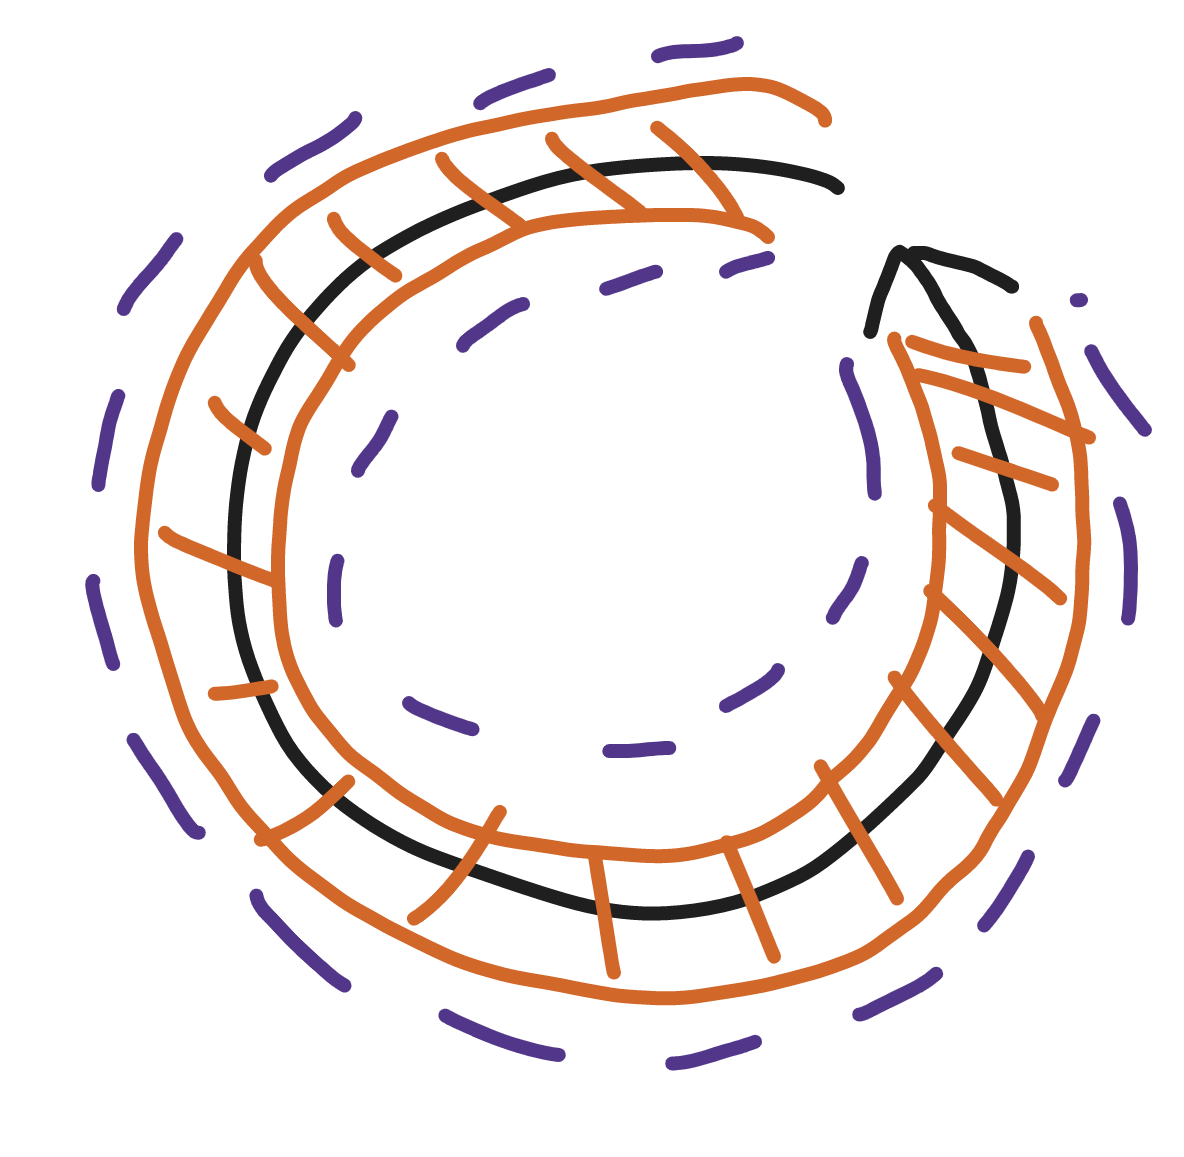
\includegraphics[]{Images/single_loop_top_down.PNG}\\
Luckily, neutrons have a non-zero magnetic moment. How much energy would such a device take, and is it better to accelerate protons instead? The purpose of using a solenoid is to allow the neutron to travel a large distance within the target medium to account for a small reaction cross section. Furthermore,the solenoid design allows the experiment to not take up a large volume for potentially km-scale travel distances. \\
Is it possible to make the neutron follow this trajectory with a singular magnetic field that works to similarly to a gravitational field? 
\subsubsection{9/6/2022}
LADWP serves 1200 km2 of area. 
it would take 10$^{10-1.5}$ = 10$^{8.5}$ m$^2$ = 300 km$^2$ of solar panels to power LA. So LA needs to cover 1/3 of the county in solar\\
Checked using google earth and solargis. \\
\includegraphics[scale=.62]{Images/solar irradiance la county screenshot.PNG}\\
\includegraphics[scale=.62]{Images/solar irradiance sf valley screenshot.PNG}
\subsubsection{9/7/2022}
If energy can be efficiently recovered from $\gamma$ rays by heating up a thick shielding, which is then connected to a thermocouple, then the following may be an energy efficient way of producing neutrons\\
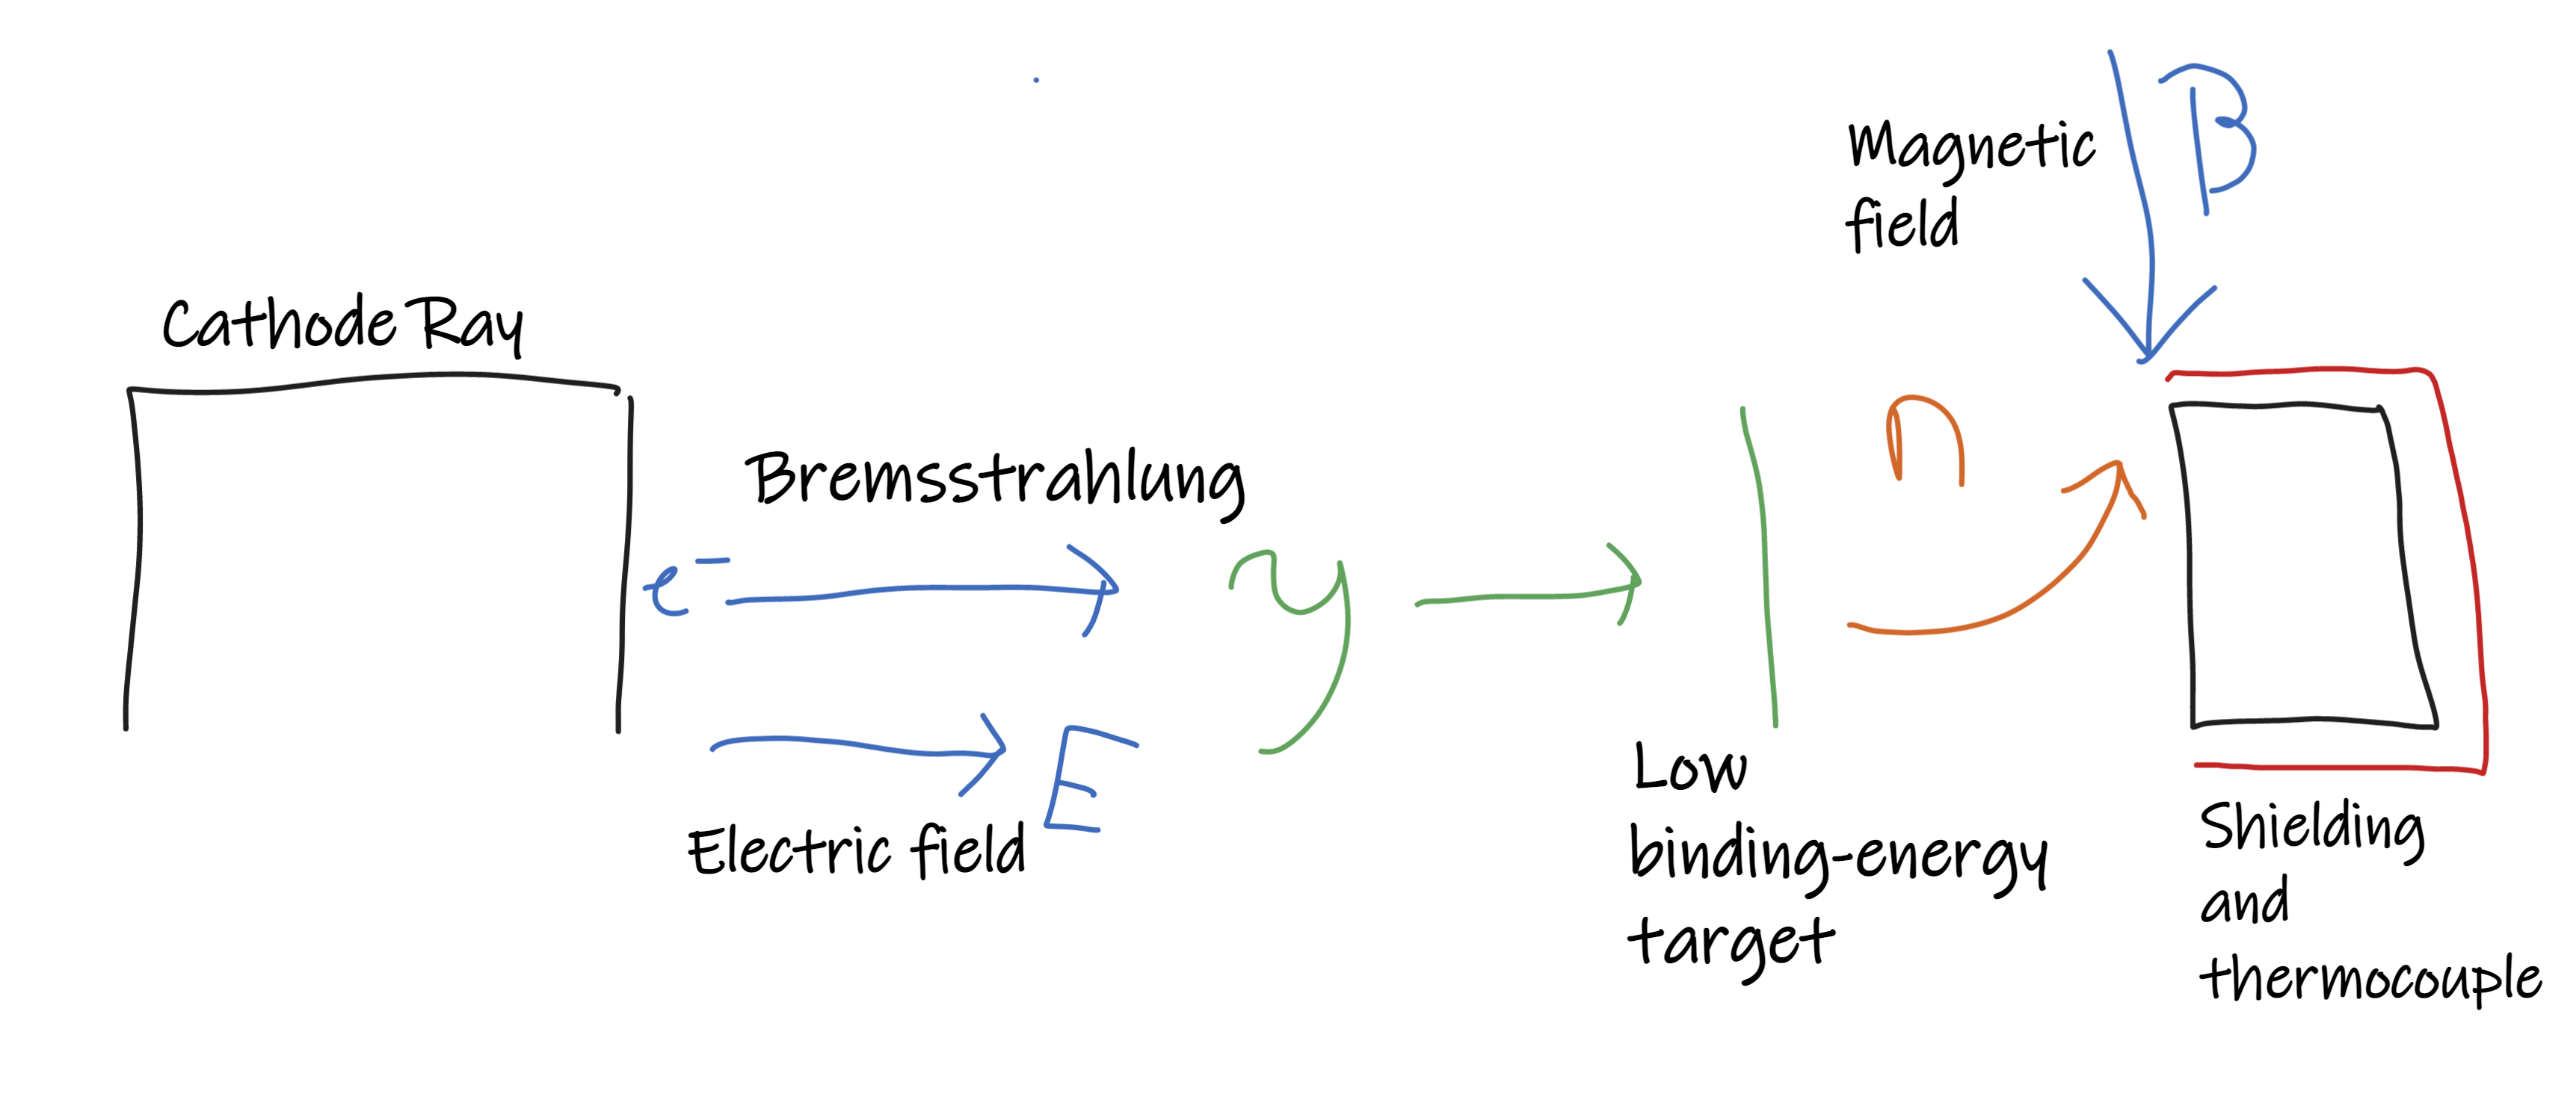
\includegraphics[scale=.65]{Images/neutron generator concept.PNG}\\
\subsubsection{9/12/2022}
Thought of a new setup for generating radioisotopes. This prioritizes energy efficiency by making use of spallation by relativistic protons. These protons are accelerated using the wake field of a plasma, which is created with laser. 
The spallation of protons onto the target releases neutrons which are then guided by a magnetic field to make many loops through a circular target to ensure a reaction. See the zotero group for more information on spallation, lasers, and neutron interactions through matter and magnetic fields. \\
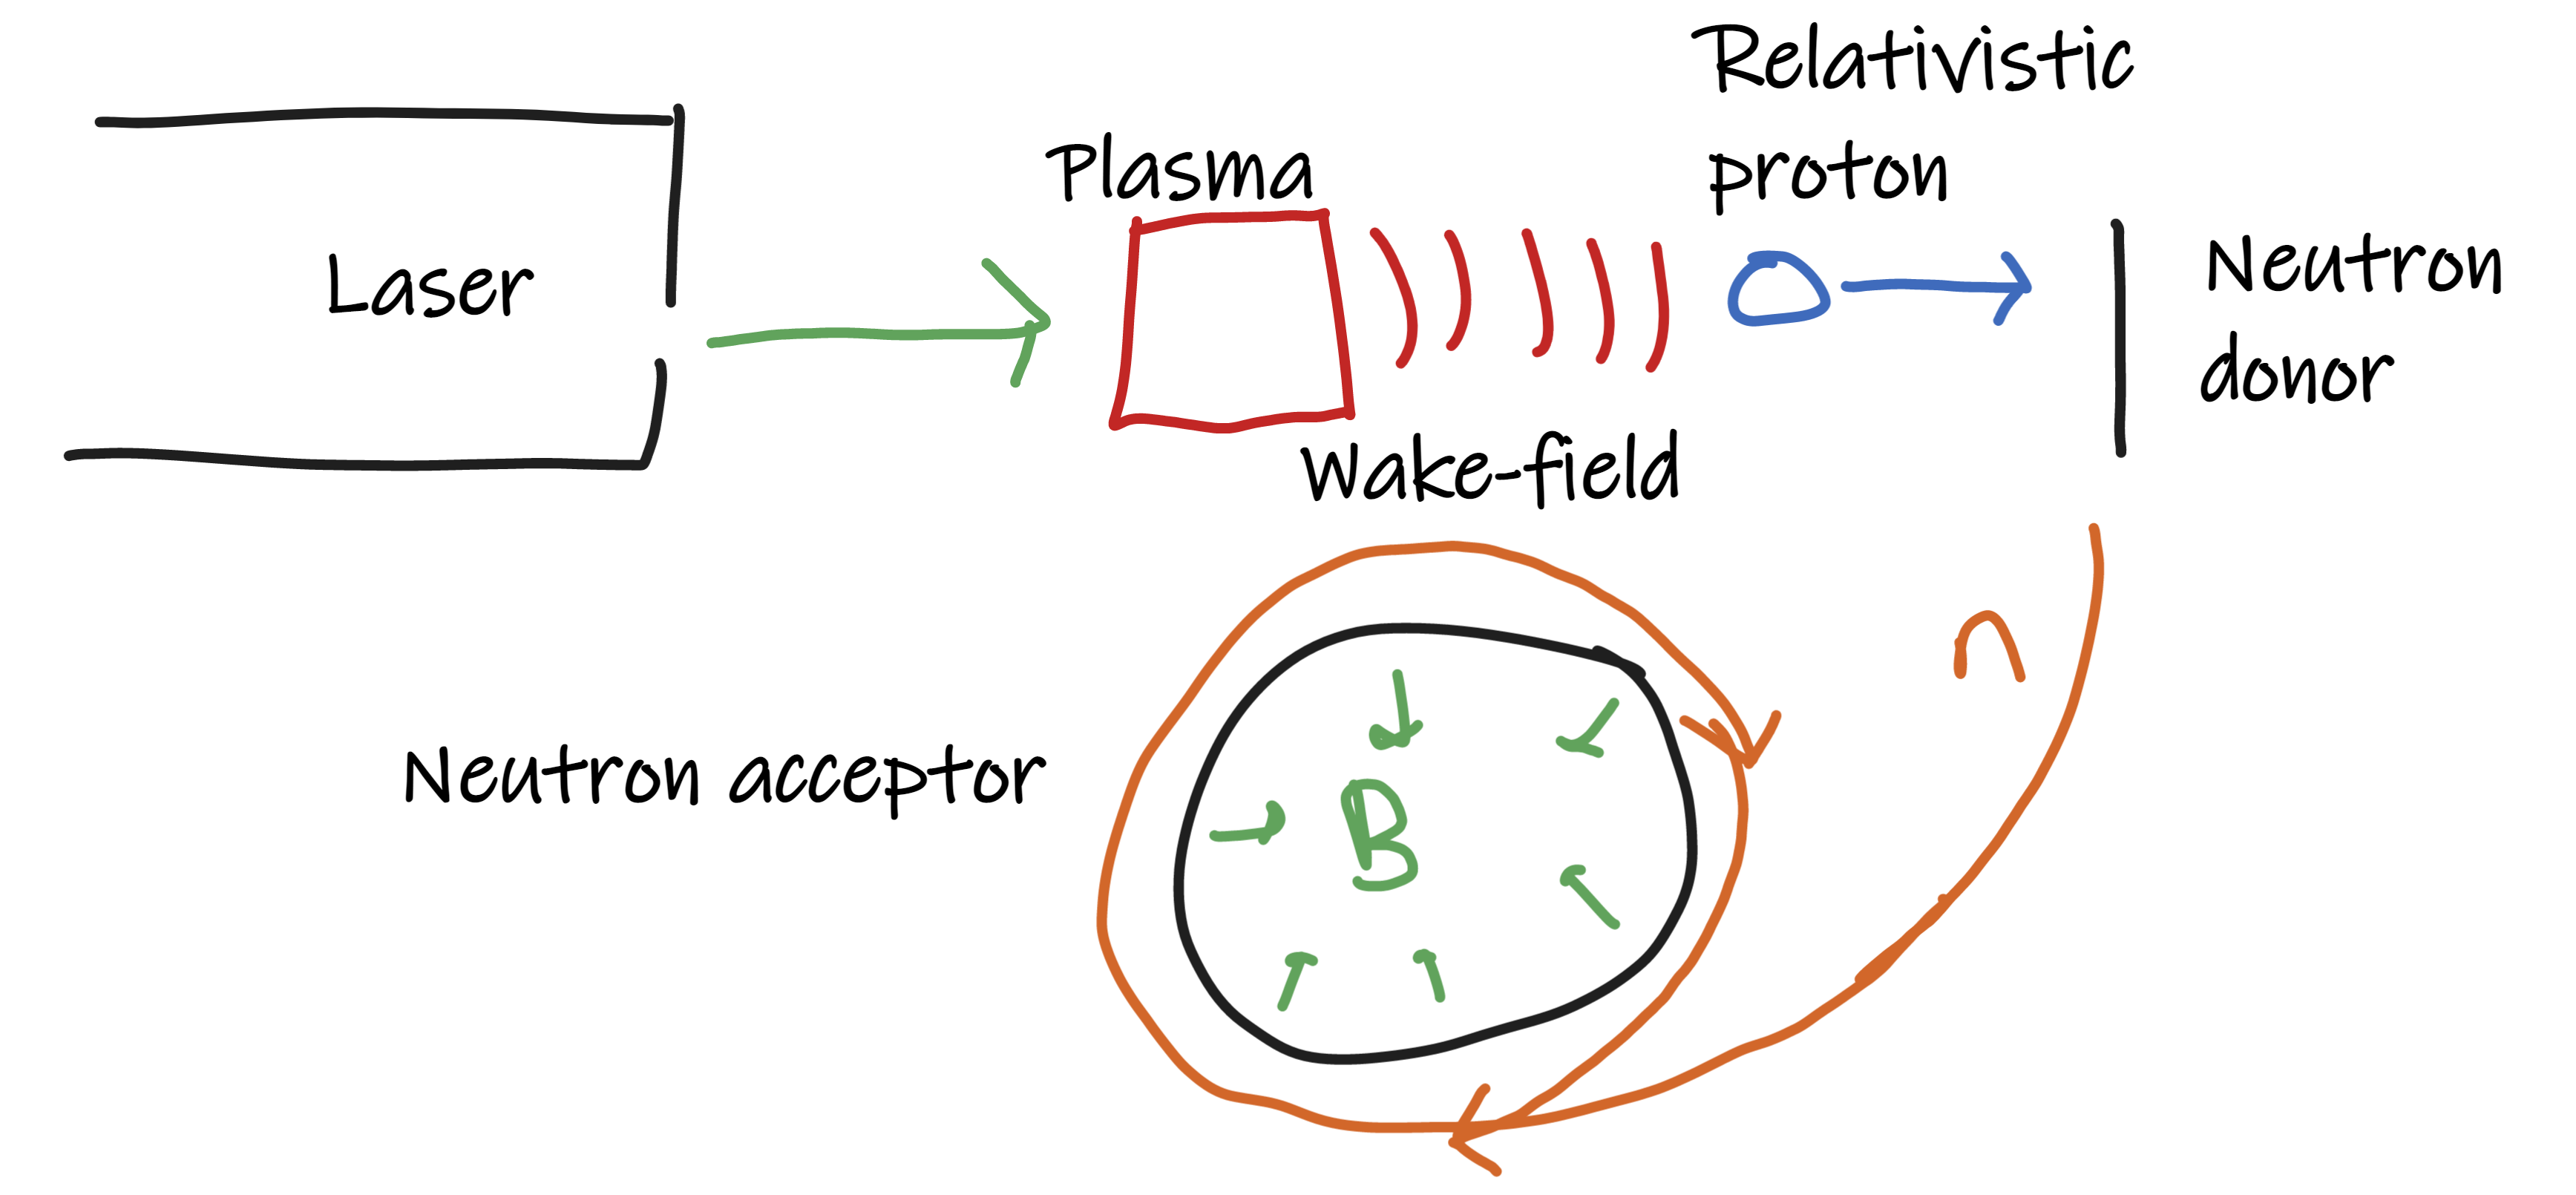
\includegraphics[scale=.65]{Images/laser plasma accelerated spallation neutron generator concept.PNG}\\
Note that a magnetic field guides the neutron through the target. \\
Now to simulate this setup. I'll call it laser plasma wakefield spallation neutron source (LPWFSNS) 
\subsubsection{9/13/2022}
Most plamsa wakefield accelerators are designed to accelerate electrons rather than protons. However, I wonder if energy efficient acceleration of protons can also be achieved. \href{http://dx.doi.org/10.1098/rsta.2019.0215}{Hidding et al. RSP. 2019} claim that separating electrons and ions within a plasma can generate electric fields on the order of TV/m, and that intense laser pulses or particles are sufficient energy sources. 
\subsubsection{9/14/2022}
Mostly reading papers on proton accelerators and calculated their energy efficiency. Accelerating a protons using an electron beam such as those produced by laser wake field particle accelerators (LWFPA) is 1000x more efficient than currently existing neutron generators. However, this would still be $<$1\% energy efficient for energy storage. \\
Consider a much simpler case, using brehmsstrahlung of electrons to produce gamma rays. The cross section of the reaction $^2$H(g,n)$ ^1$H is on the order of 10$^-2.5$b $= 10^{-30.5}$m$^2$ for 4.5 MeV $\gamma$ rays. We have for the probability of the reaction 
\begin{equation}
\begin{split}
\\
\end{split}
\end{equation}
\subsubsection{9/15/2022}
I should take into greater account the energy consumed and produced in nuclear reactions. \\
Would stripping all of the electrons from an atom that can only decay by electron capture stop it from decaying? If so, this seems like an effective way to control the decay radioisotopes.\\
From the Rydberg formula, an atom's ionization energy is proportional to $Z^2$. This gives a maximum of 13,000x larger than hydrogen's ionization energy of 13 eV. This assumes that all electrons are held at the same radii, which they aren't. 
Found some ionization energies here: https://webbook.nist.gov/chemistry/ie-ser/ and https://physics.nist.gov/PhysRefData/ASD/ionEnergy.html and https://physics.nist.gov/cgi-bin/ASD/ie.pl in case I need them later. 




\end{document}
